\chapter{二维材料异质结生长机理的研究}
\section{引言}
石墨烯作为经典的二维材料,由于独特的晶体结构和电子结构特性,在超导,量子计算、量子晶体管等方面具有独特的优势\citing{RN1068-2020,RN1071-2021,RN1065-2013,RN997-2007,RN1008-2015}。而要将石墨烯与现行集成电路使用的平面硅工艺兼容,需要将石墨烯转移到\cemb{SiO2}等绝缘衬底的表面。而石墨烯在\cemb{SiO2}等绝缘衬底表面通常以无序的状态存在,破碎的晶格使得石墨烯在这些绝缘衬底的表面难以完全发挥出理论上限。

而作为二维材料中的绝缘体,六方氮化硼\cemb{h-BN}在具有较大的带隙的同时也保有二维材料高质量面内结构的特点。趋近完美的二维晶体结构使得\cemb{h-BN}在禁带内具有极低的缺陷态密度以及较高的击穿电压。同时,\cemb{h-BN}与石墨烯之间的晶格失配只有\SI{2}{\percent},这使得\cemb{h-BN}非常适合搞高性能电子器件中替代\cemb{SiO2}作为石墨烯的衬底材料 \citing{RN959-2010}。这种将不同的二维材料纵向堆叠起来可以制成纵向异质结,层与层之间由较弱的范德华力或准范德华力连接。以二维材料所组成的异质结能够结合不同二维材料优异的物理特性,使得二维材料在多种新型器件中能够最大化的发挥其独特的优势。许多新奇的物理现象已经在石墨烯和\cemb{h-BN}的纵向堆叠而成的二维异质结被研究者所发现,如在外磁场下电子和磁场场强的霍夫斯塔特蝴蝶分型图像\citing{RN1286-2013, RN1287-2013, RN1285-2013}。同时,石墨烯/\cemb{h-BN}纵向二维异质结具有非常好的制备质量,石墨烯高度可调的物理特性,以及二者之间存在的周期性的摩尔超晶格。这些都使得石墨烯/\cemb{h-BN}纵向二维异质结成为了一个非常好的观测新奇量子现象的基础平台。

然而,虽然机械剥离的方式能够制备具有极高质量的石墨烯/\cemb{h-BN}纵向二维异质结,但受限于较低生产效率和高昂的合成成本,剥离的方式很难应用于大规模的二维材料的生产制备。而常用于大规模低成本制备石墨烯的化学气相沉积法通常需要\cemb{Cu}等金属衬底的催化作用的协助。由于\cemb{h-BN}对于甲烷等含碳前驱体裂解反应的催化活性远不及金属衬底,石墨烯在\cemb{h-BN}上直接生长的速率同样也远低于在金属衬底上的生长速率。因此,一些研究者试图通过增加前驱体裂解速率的方式提升纵向二维异质结的合成效率。例如,在2013年,研究者发现通过等离子体辅助的方式能够在低温的环境下在\cemb{h-BN}的表面生长石墨烯\citing{RN1289-2013}。在2015年,研究者通过添加作为气体催化剂的硅烷等方式,可以促进甲烷的裂解,提高石墨烯在\cemb{h-BN}表面的生长速率\citing{RN1059-2015}。但以上方式通常使用剥离的\cemb{h-BN}作为石墨烯的生长衬底,使用较高的生长温度或者使用等离子体辅助的方式进行生长。在这种情况下,虽然石墨烯能够在\cemb{h-BN}的表面生长,但是高温会破坏金属衬底,而\cemb{h-BN}本身的生长需要在金属衬底的表面。因此我们需要寻找到一种生长流程,使得温度维持在金属衬底能够生长\cemb{h-BN}能够的同时,尽可能的加快石墨烯在\cemb{h-BN}表面的生长速率。

在\ref{cap:CG}章中,我们构建了一种利用\cemb{Cu}蒸气近邻催化效应在\cemb{h-BN}表面直接堆叠生长石墨烯的方法。该方法利用从外缘\cemb{Cu}源处蒸发而出的\cemb{Cu}蒸气作为催化剂,在\cemb{h-BN}的表面产生对\cemb{CH4}的近邻催化效应,加速甲烷在\cemb{h-BN}表面的裂解,从而达到加速\cemb{h-BN}表面石墨烯生长的目的。利用理论计算的方法,我们证明了\cemb{Cu}蒸气从蒸发源到达\cemb{h-BN}表面并进行\cemb{CH4}裂解催化的可行性,同时给出了裂解而成的碳原子在\cemb{h-BN}表面成核生长成石墨烯的生长序列。我们认为通过这种直接堆叠生长的方法能够能够实现石墨烯/\cemb{h-BN}的双层以及多层堆叠交替大规模生长,进一步提升石墨烯/\cemb{h-BN}二维纵向异质结在高性能电子器件应用的可行性,推进石墨烯/\cemb{h-BN}二维纵向异质结的工程化和集成化。

\section{计算细节}

在本章中密度泛函理论主要使用Vienna ab-initio Simulation Package (VASP) 软件包进行计算。在密度泛函理论计算中,我们使用广义梯度近似(GGA)下的 Perdew-Burke-Ernzerhof (PBE)泛函描述电子之间的交换关联作用。平面波的截断动能取为为$\SI{500}{\electronvolt}$。为了研究\cemb{Cu}/\cemb{h-BN}衬底表面石墨烯的生长情况,我们采用切片模型并在垂直表面方向放置至少$\SI{20}{\angstrom}$的真空层以防止周期性条件相邻切片的影响。切片模型中,作为石墨烯生长衬底的\cemb{Cu}/\cemb{h-BN}包含四原子层的\cemb{Cu(111)}以及单原子层的\cemb{h-BN}。在\cemb{Cu}的表面,经过我们的计算,\cemb{h-BN}的最优堆叠方式为\cemb{N}原子位于\cemb{Cu}衬底的顶位,\cemb{B}原子位于\cemb{Cu}衬底的面心立方位(fcc site)。
在原子结构优化的计算中,力收敛条件设为$\SI{2e-2}{\electronvolt \per \angstrom}$,电子结构自洽场计算的收敛条件设为$\SI{1e-6}{\electronvolt}$。
对于碳团簇(\cemb{C_x})、石墨烯、\cemb{h-BN}、\cemb{Cu}衬底之间之间的范德瓦尔斯作用使用Grimme的DFT-D3方法进行描述,并带有Becke-Johnson阻尼作用 \citing{RN937-2010, RN938-2011}。
对于过渡态的计算,我们采用CI-NEB(Climbing Image Nudged Elastic Band)方法对始末反应状态之间的能量鞍点进行搜寻,以确定反应势垒的大小\citing{RN790-2000}。对于过渡态计算,力收敛条件设为$\SI{3e-2}{\electronvolt \per \angstrom}$。

\section{石墨烯/\cemb{h-BN}纵向二维异质结的生长机理}
    \label{cap:CG}
    \begin{figure}[htb]
        \subfloat[]{
            \centering
            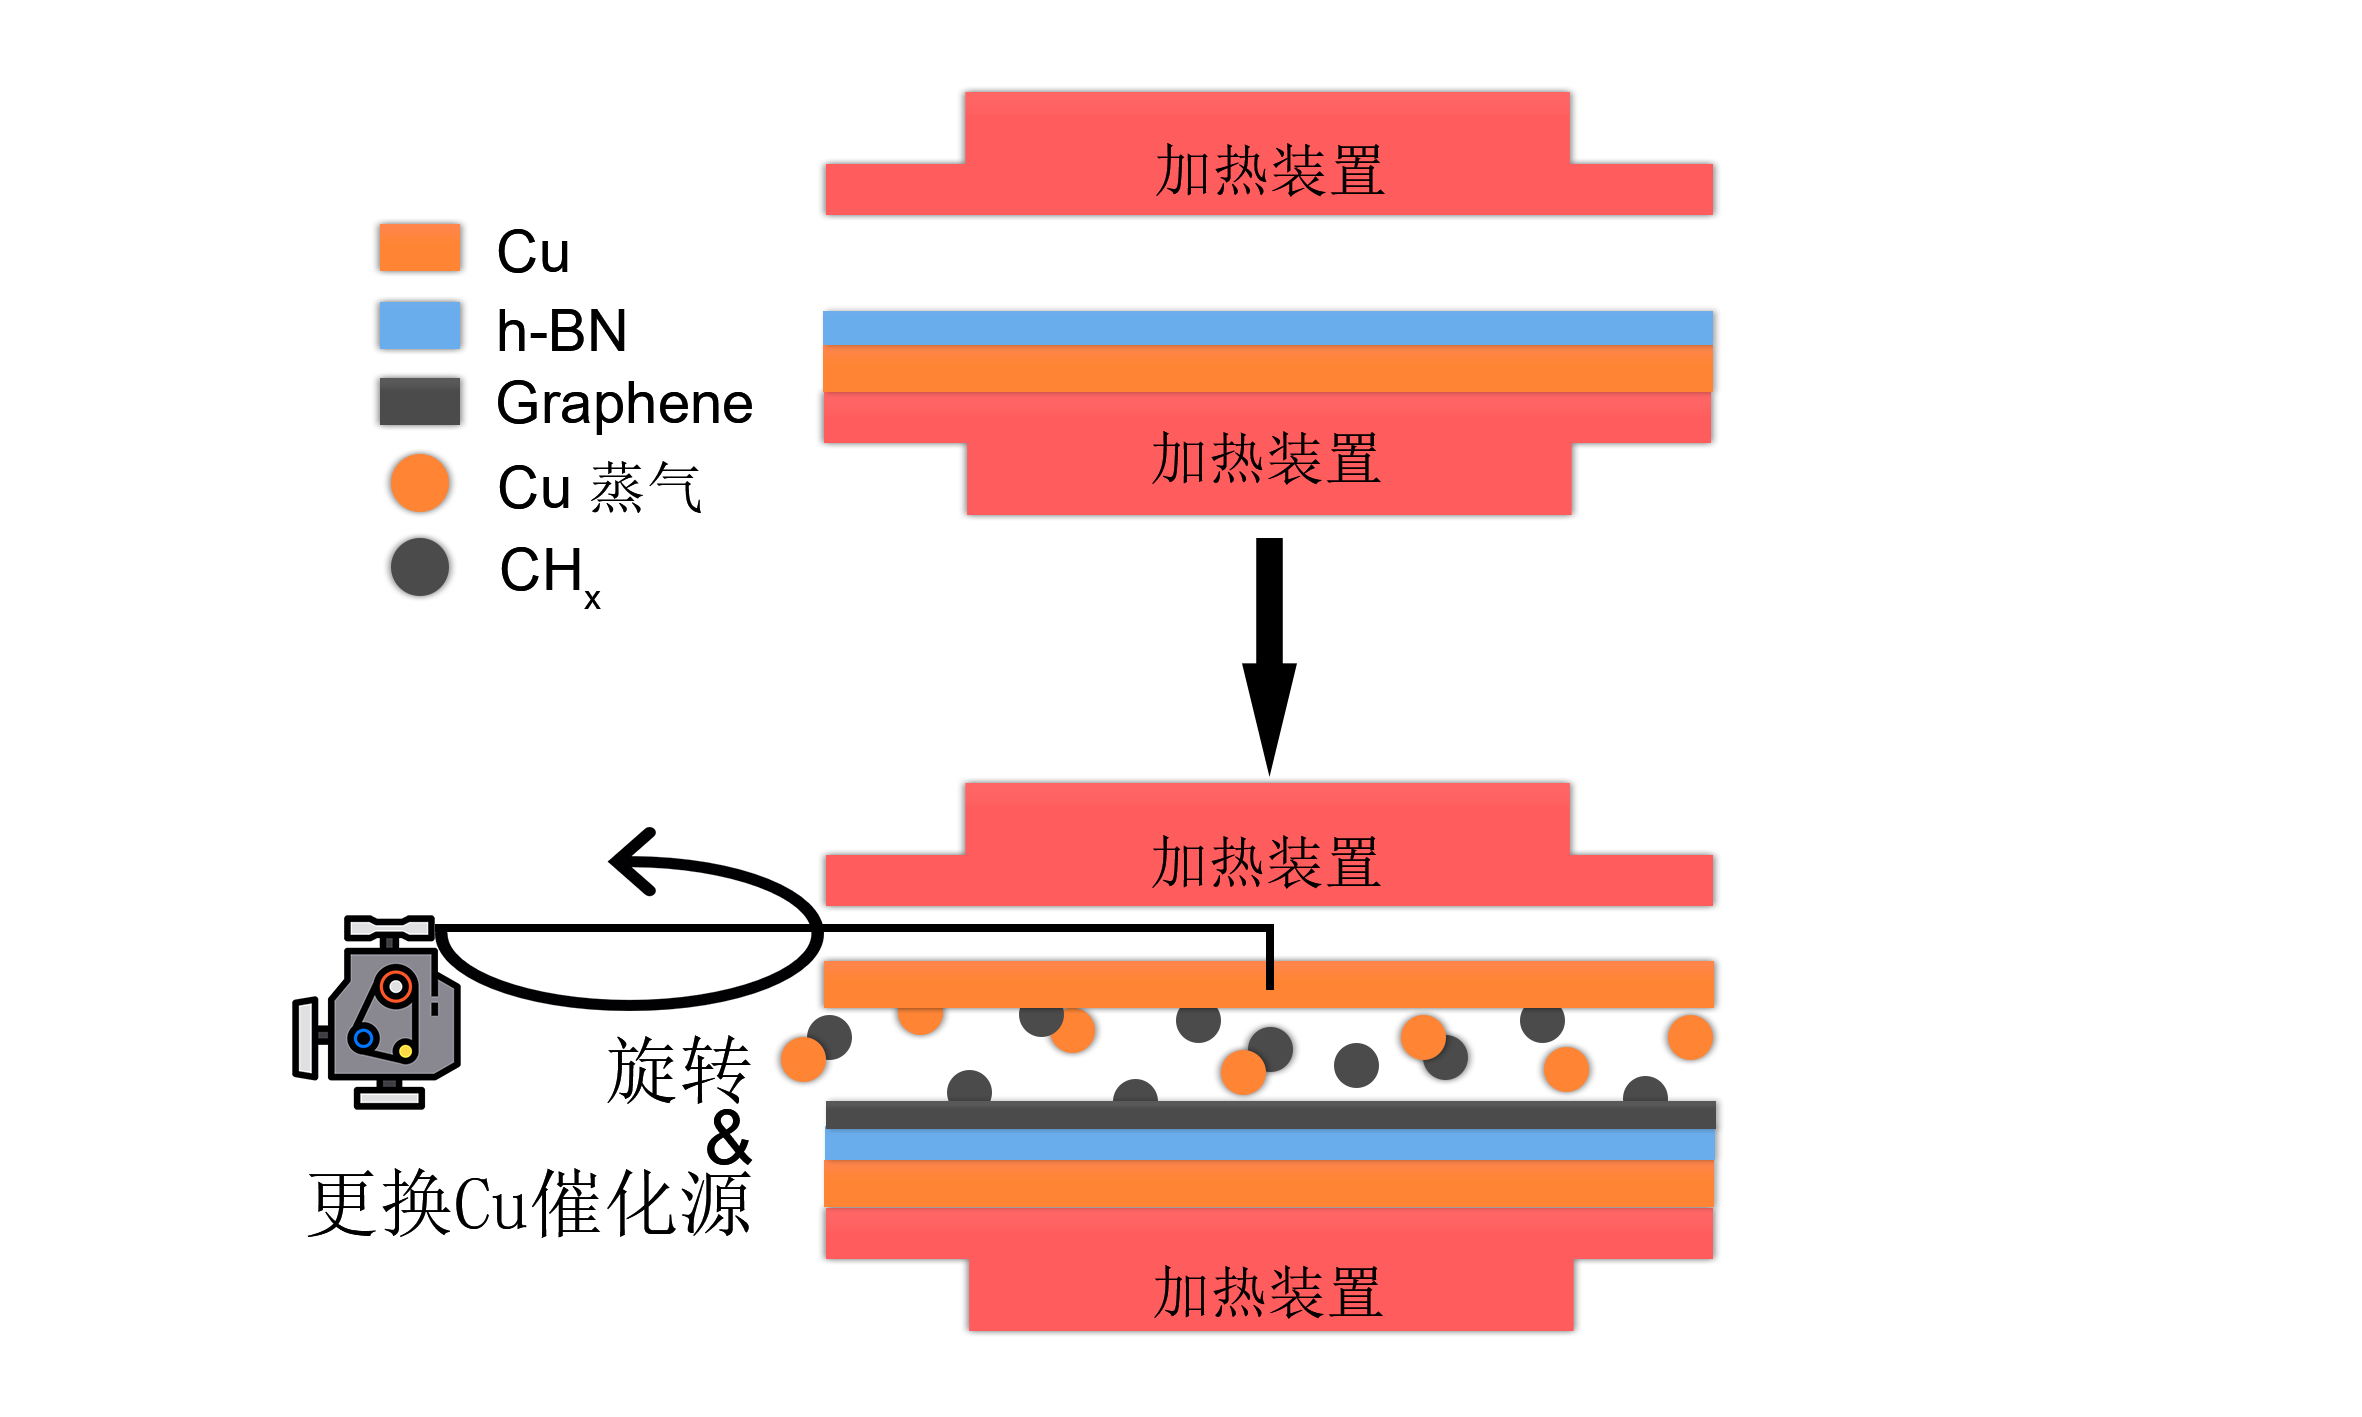
\includegraphics{pic/CG_diagram_routine.png}
            \label{fig:CG_diagram_routine}
        }
        \newline
        \subfloat[]{
            \includegraphics{pic/CG_diagram_growthSketch.png}
            \label{fig:CG_diagram_growthSketch}
        }
        \caption{利用\cemb{Cu}蒸气近邻催化效应在\cemb{h-BN}表面直接堆叠生长石墨烯。(a)生长装置示意图;(b)石墨烯/\cemb{h-BN}异质结生长过程示意图}
        \label{fig:CG_diagram_CVD}
    \end{figure}

    \subsection{近邻蒸发气态\cemb{Cu}催化剂的扩散}
    
    \begin{figure}[htb]
        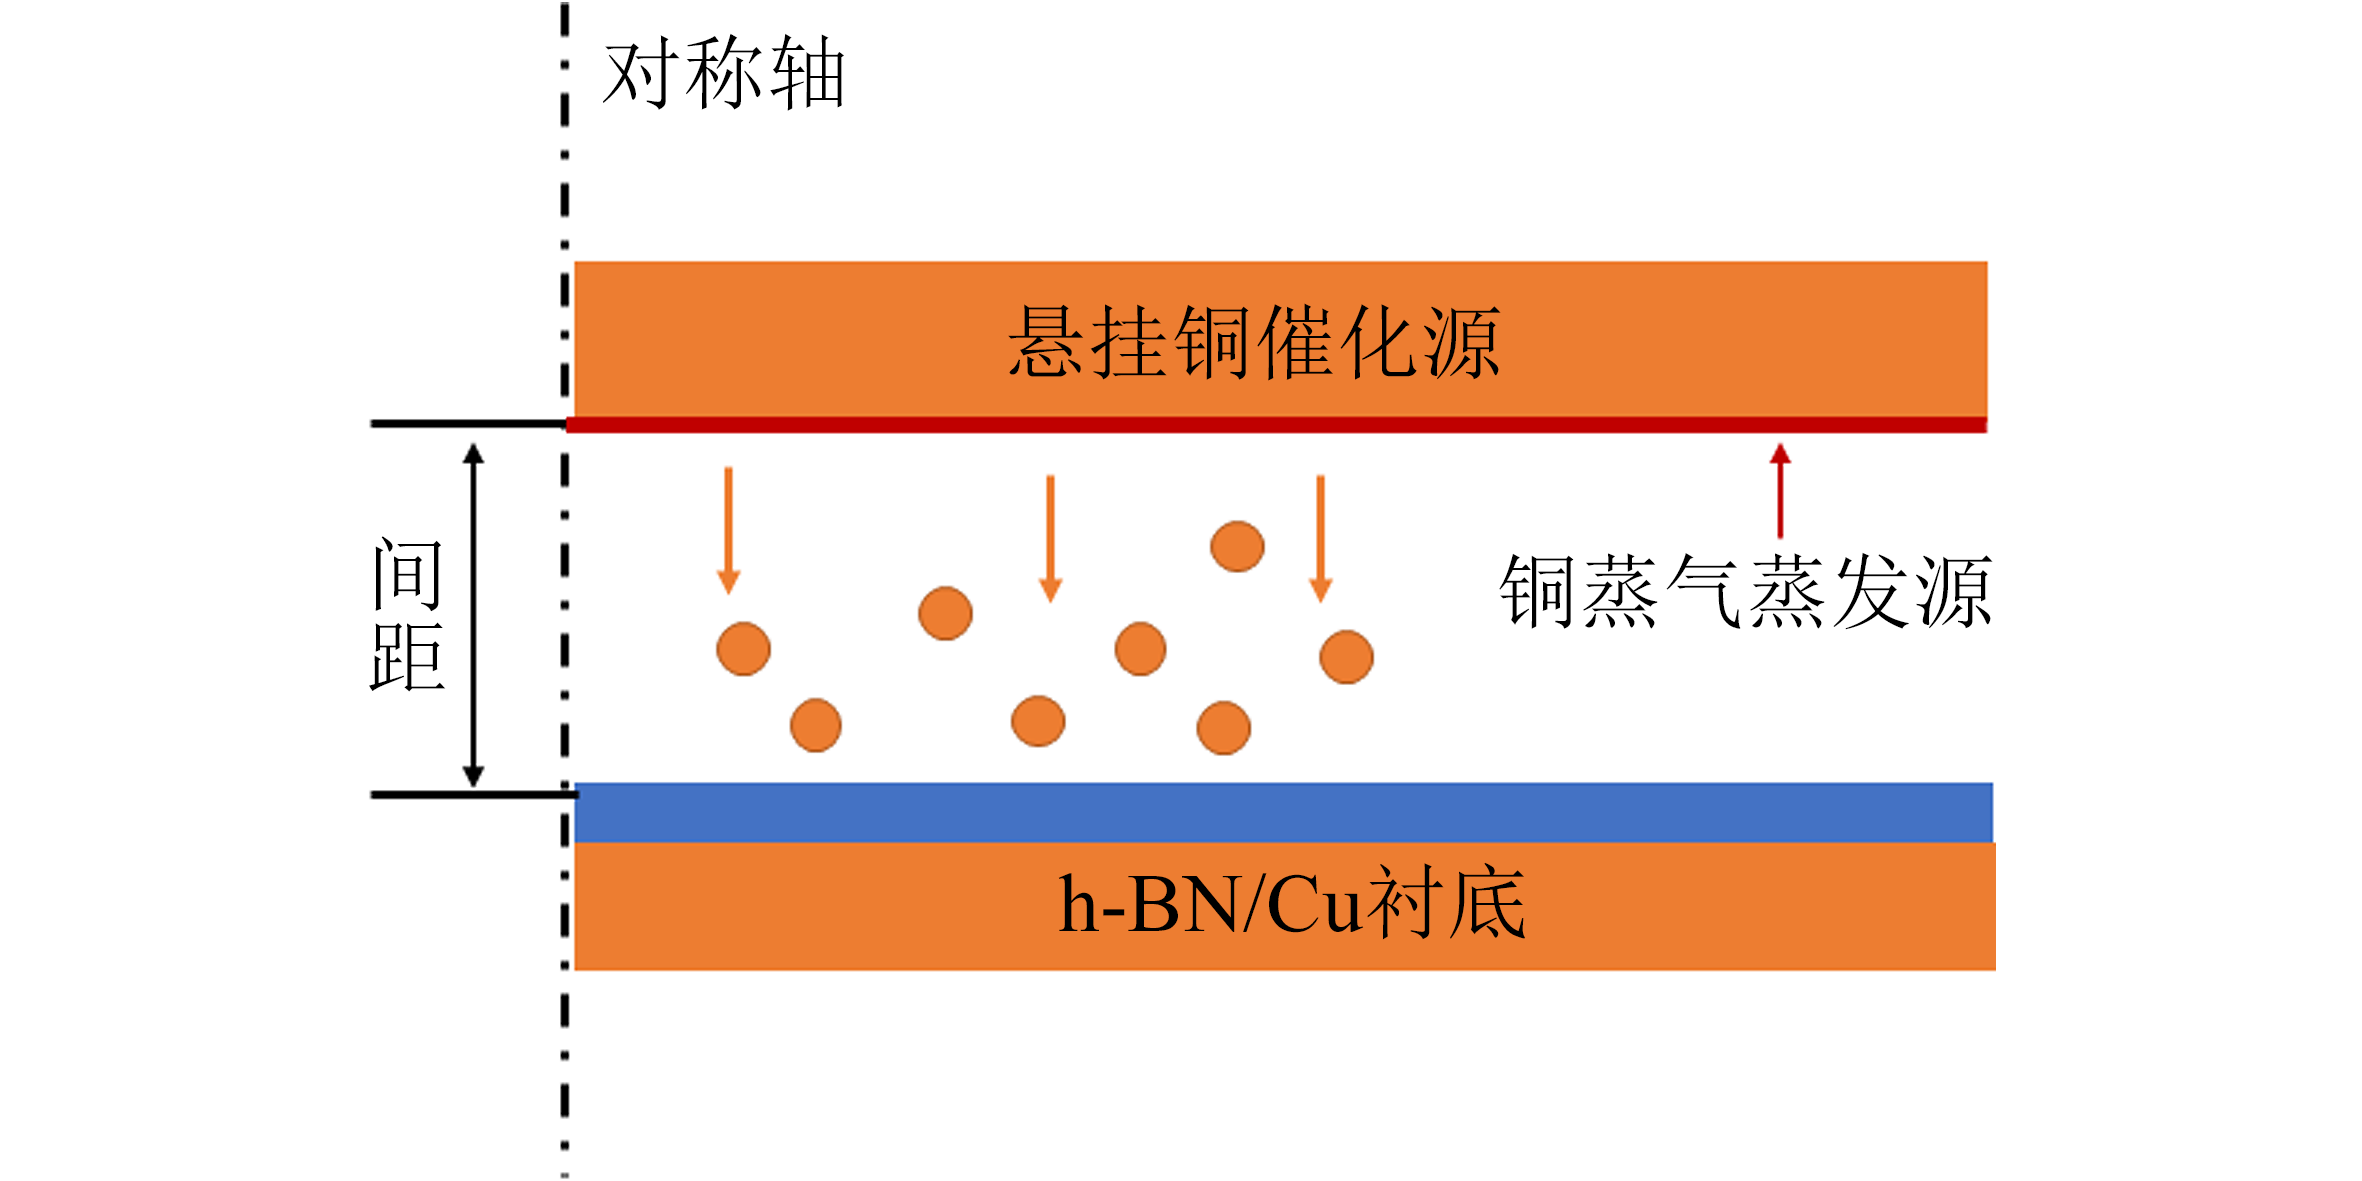
\includegraphics{pic/CG_diagram_FEM_structure.png}
        \caption{化学气相沉积腔体内\cemb{Cu}蒸气扩散模拟示意图。}
        \label{fig:CG_diagram_FEM_structure}
    \end{figure}

    \begin{figure}[htb]
        
    \end{figure}

    \subsection{气态\cemb{Cu}催化剂对甲烷裂解反应的催化性能}
    \subsection{\cemb{h-BN}表面石墨烯的生长演化机理}
\section{石墨烯/二硒化钒横向异质结的生长机理}
\section{总结}